\let\negmedspace\undefined
\let\negthickspace\undefined
\documentclass[journal]{IEEEtran}
\usepackage[a5paper, margin=10mm, onecolumn]{geometry}
%\usepackage{lmodern} % Ensure lmodern is loaded for pdflatex
\usepackage{tfrupee} % Include tfrupee package

\setlength{\headheight}{1cm} % Set the height of the header box
\setlength{\headsep}{0mm}     % Set the distance between the header box and the top of the text
\usepackage{verbatim}
\usepackage{gvv-book}
\usepackage{hyperref}
\usepackage{gvv}
\usepackage{cite}
\usepackage{amsmath,amssymb,amsfonts,amsthm}
\usepackage{algorithmic}
\usepackage{graphicx}
\usepackage{textcomp}
\usepackage{xcolor}
\usepackage{txfonts}
\usepackage{listings}
\usepackage{enumitem}
\usepackage{mathtools}
\usepackage{gensymb}
\usepackage{comment}
\usepackage[breaklinks=true]{hyperref}
\usepackage{tkz-euclide} 
\usepackage{listings}
% \usepackage{gvv}                                        
\def\inputGnumericTable{}                                 
\usepackage[latin1]{inputenc}                                
\usepackage{color}                                            
\usepackage{array}                                            
\usepackage{longtable}                                       
\usepackage{calc}                                             
\usepackage{multirow}                                         
\usepackage{hhline}                                           
\usepackage{ifthen}                                           
\usepackage{lscape}
\usepackage{circuitikz}
\usepackage{titlesec}
\usepackage{placeins}
\usepackage{pgfplots}
\usepackage{xcolor}
\usepackage{tikz}
\usepackage{listings}
\usepackage{xcolor}
\usepackage{tcolorbox}
\tikzstyle{block} = [rectangle, draw, fill=blue!20, 
    text width=4em, text centered, rounded corners, minimum height=3em]
\tikzstyle{sum} = [draw, fill=blue!10, circle, minimum size=1cm, node distance=1.5cm]
\tikzstyle{input} = [coordinate]
\tikzstyle{output} = [coordinate]
\titleformat{\section}[hang]{\normalfont\bfseries}{\thesection}{1em}{}


\usepackage{graphicx}
\usepackage{amsmath}
\usepackage{listings}
\usepackage{xcolor}

\lstdefinestyle{customC}{
    language=C,
    basicstyle=\ttfamily\footnotesize,
    keywordstyle=\color{blue}\bfseries,
    commentstyle=\color{green!50!black},
    stringstyle=\color{red!70!black},
    numbers=left,
    numberstyle=\tiny\color{gray},
    stepnumber=1,
    breaklines=true,
    frame=single,
    tabsize=4
}


\begin{document}

\begin{titlepage}
    \centering
    {\Huge \bfseries Digital Clock

 \par}
    \vspace{2cm}

   
    {\Large \bfseries Hardware Project \par}
    \vspace{0.5cm}
   
    {\large EE1003 : Scientific Programming \par}
    \vspace{1cm}
    {\large GVV Sharma\par}
    \vspace{3cm}
\begin{tabular}{ll}
    \textbf{Harshil Rathan Y } & \textbf{EE24BTECH11064} \\
\end{tabular}
\end{titlepage}
\newpage
\tableofcontents
\newpage

\bibliographystyle{IEEEtran}
\vspace{3cm}

\renewcommand{\thefigure}{\theenumi}
\renewcommand{\thetable}{\theenumi}
\setlength{\intextsep}{10pt} % Space between text and floats


\numberwithin{equation}{enumi}
\numberwithin{figure}{enumi}
\renewcommand{\thetable}{\theenumi}
\section{Introduction}
This project implements a real time 24-hour clock using an Arduino, 7-segment displays and a 7447 BCD decoder using boolean logic. The clock displays hours, minutes and seconds using the time keeping logic iin avr-gcc 
\section{Components Required}
\begin{itemize}
    \item[1.] Arduino UNO - 1 
    \item[2.] 7 Segment Display - 6 
    \item[3.] 7447 IC - 1 
    \item[4.] Breadboard - 2 
    \item[5.] Jumper cables 
    \item[6.] Push Buttons  
\end{itemize}
\section{Circuit Design}
\subsection{Pin Diagrams}
The pin-out diagram of a 7 segement display is given below, in this project we used 6 displays for HH : MM : SS format
\begin{figure}[H]
    \centering
    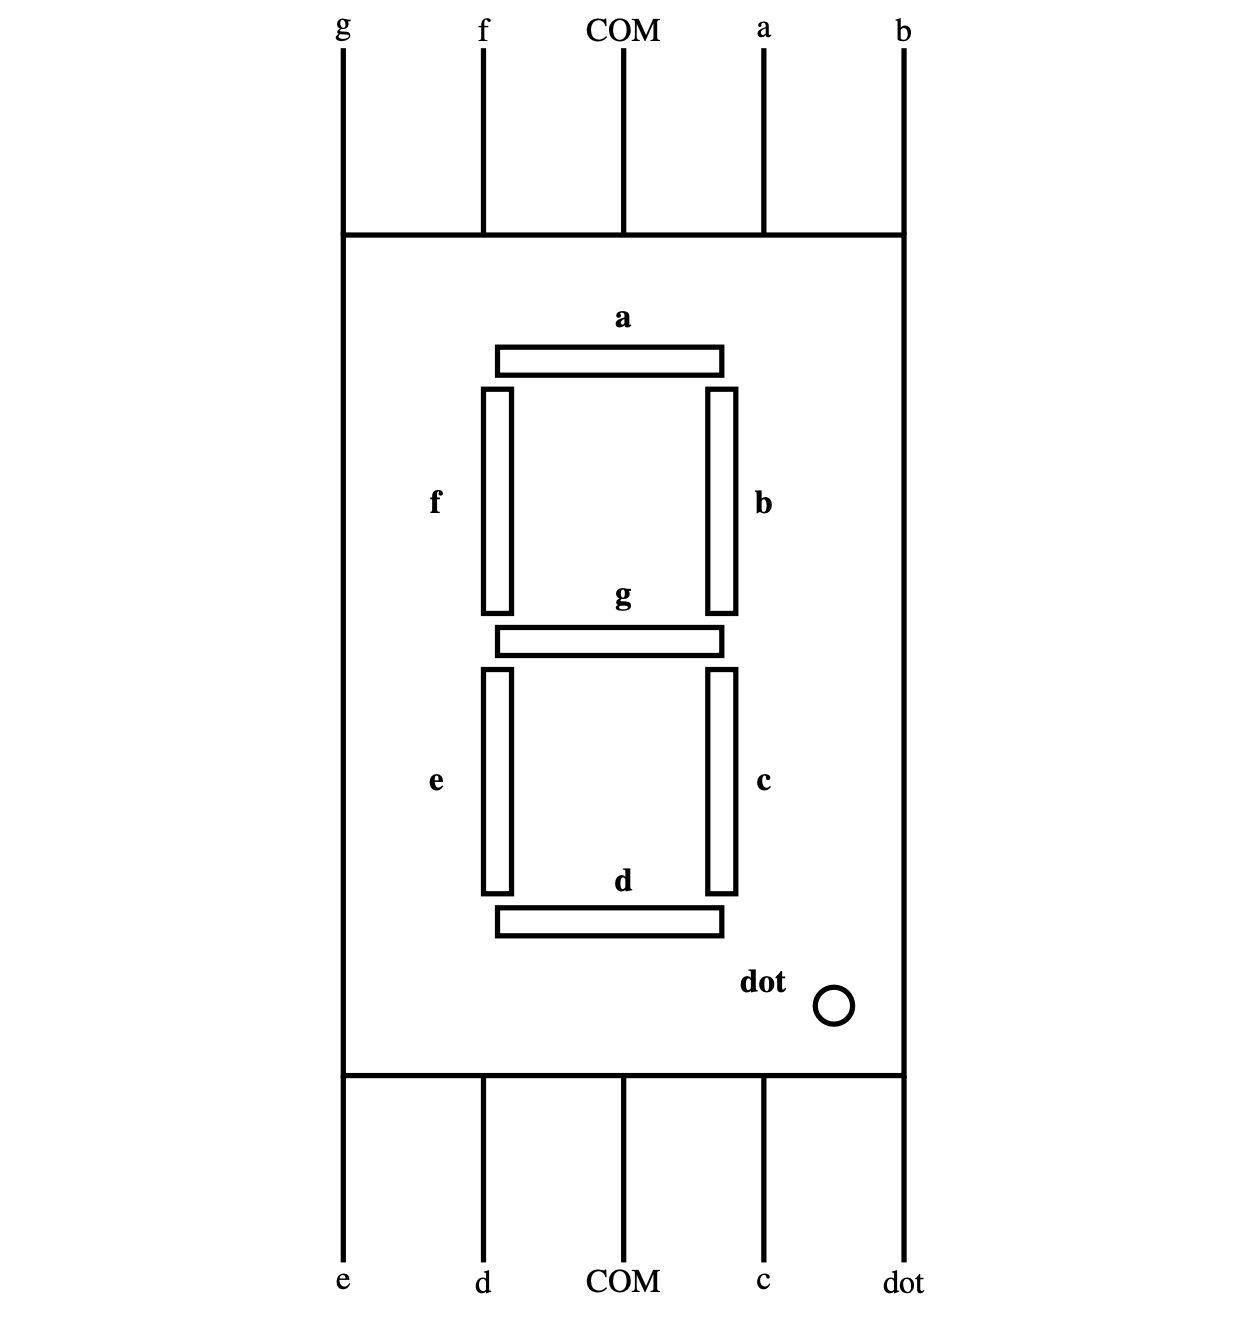
\includegraphics[width=0.3\linewidth]{figs/sevensegPinout.png}
\end{figure}
The pin-out diagram of a 7447 Decoder is below 
\begin{figure}[H]
    \centering
    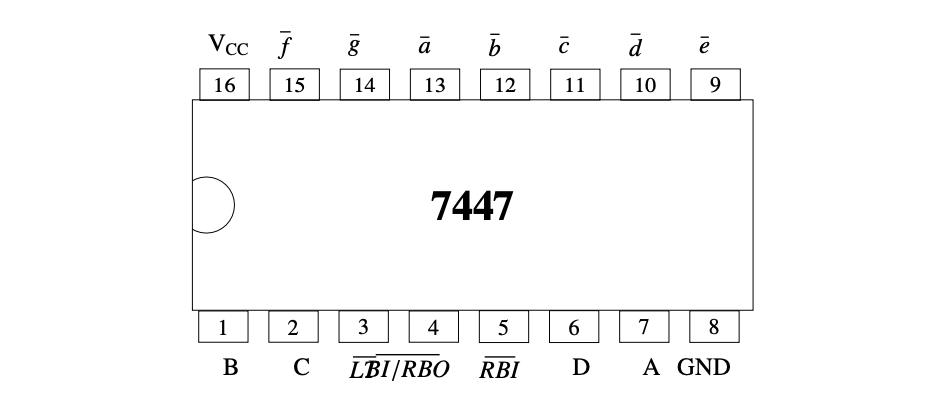
\includegraphics[width=0.4\linewidth]{figs/pinout.png}
\end{figure}
\subsection{Multiplexing}
\subsection*{Why is Multiplexing used}
\begin{itemize}
    \item Multiplexing is a method of controlling multiple displays by activating only one display at a time while rapidly switching between them. This creates an illusion of all displays being lit simultaneously due to persistence of vision in human eyes.
    \item Here we used it to control 6 displays with just one 7447 BCD decoder since the Arduino has a limited number of pins.
\end{itemize}
\subsection*{Connections}
\begin{itemize}
    \item Connect all corresponding segment pins (a-g) of the 7-segment displays to their respective output pins (13, 12, 11, 10, 9, 15, 14) on the 7447 IC
\end{itemize}
Make connections accordingly 
\begin{figure}[H]
    \centering
    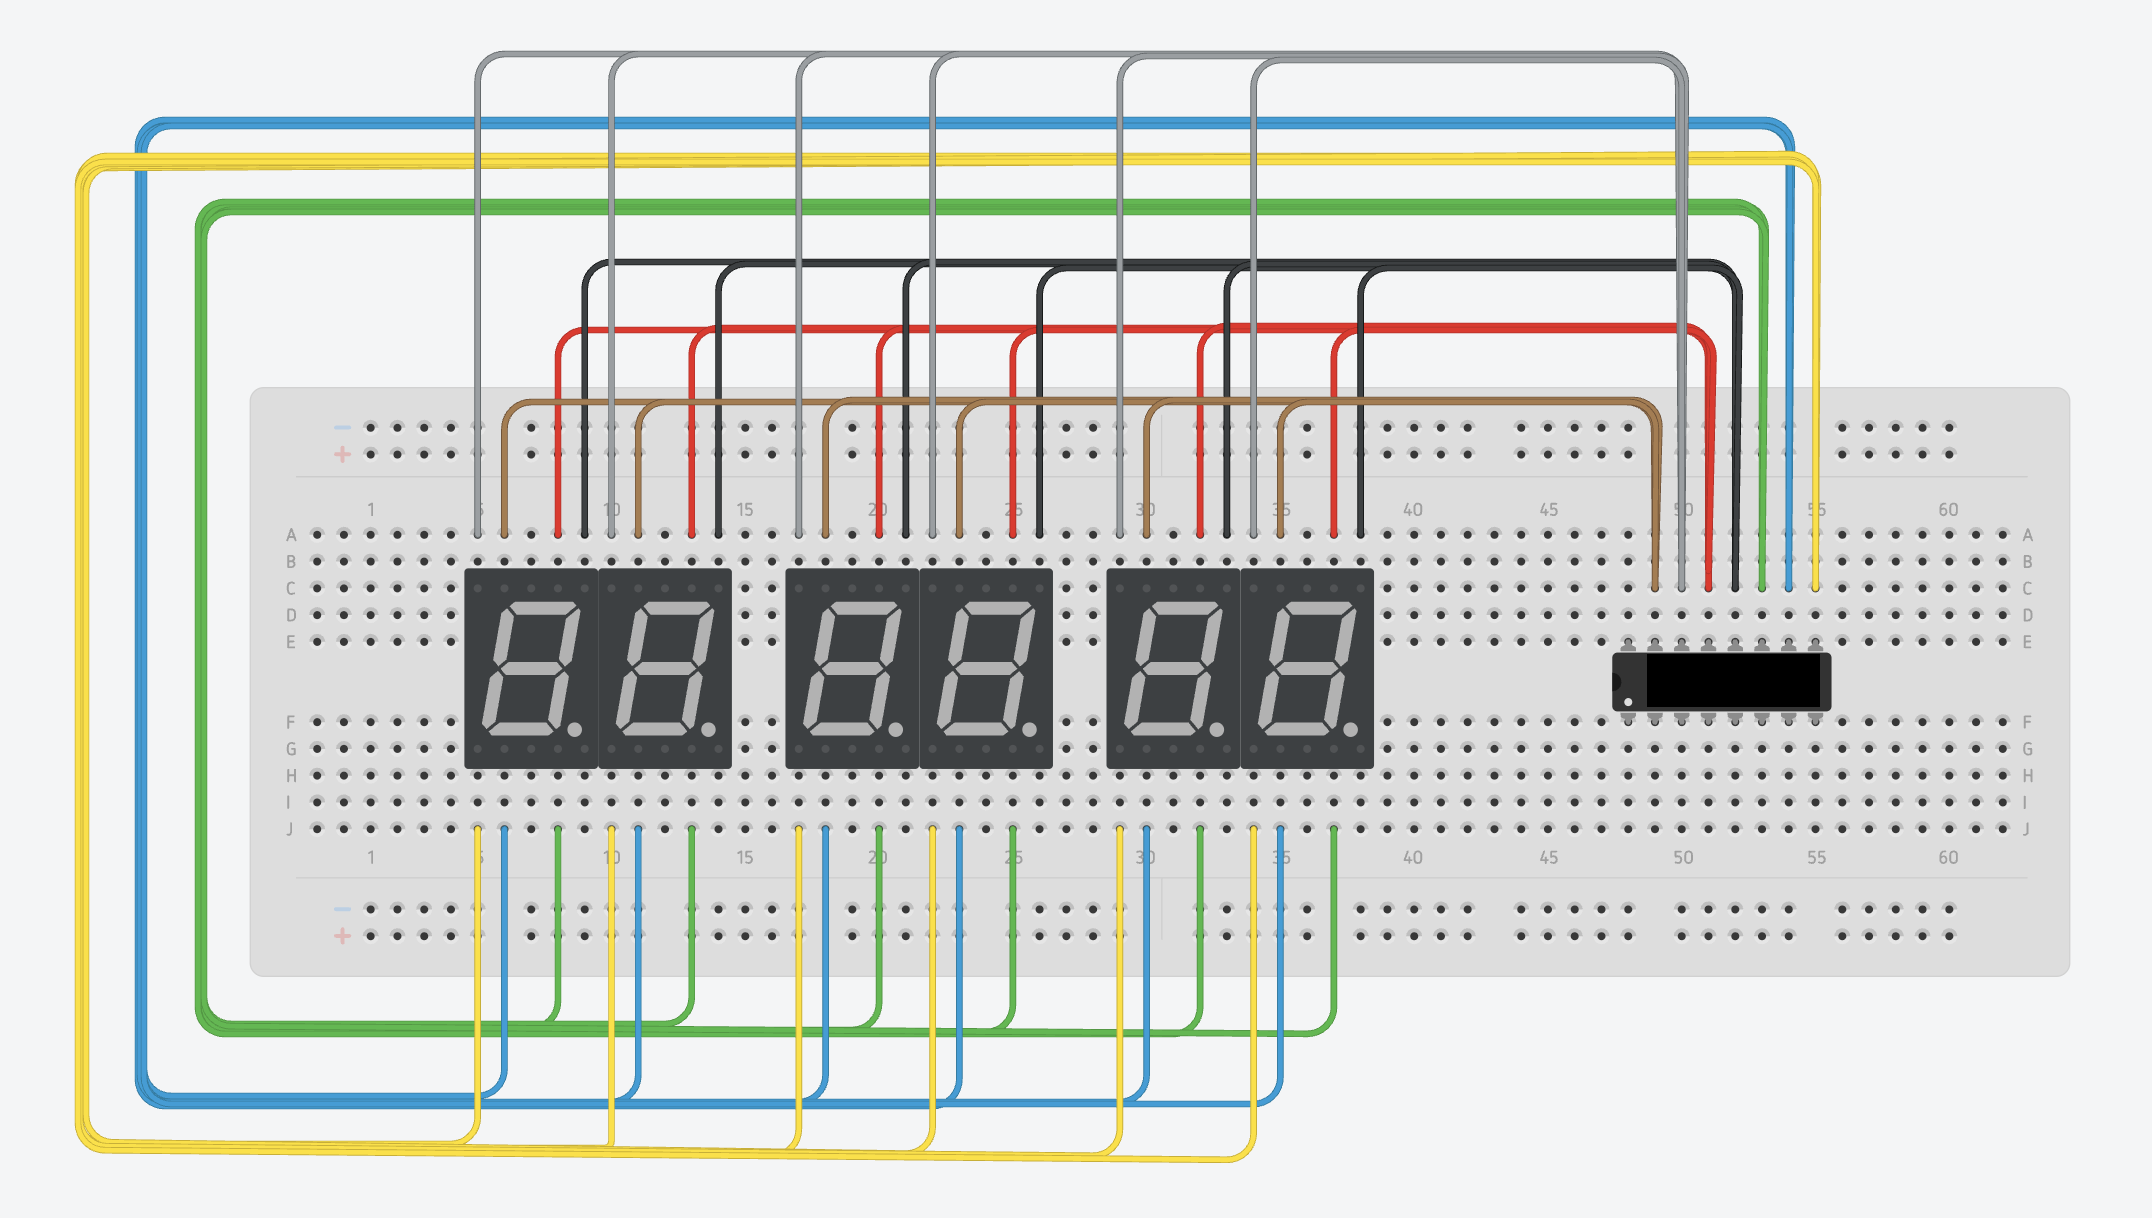
\includegraphics[width=0.8\linewidth]{figs/multiplexing .png}
\end{figure}

Follow thesd further connections \\
\begin{table}[H]
    \centering
    \begin{tabular}{|c|c|c|}
        \hline
        \textbf{Connections} & \textbf{7447 Pins} & \textbf{Arduino Pin} \\
        \hline
        BCD A & Pin 7 & D2 (PD2) \\
        BCD B        & Pin 1 & D3 (PD3) \\
        BCD C        & Pin 2 & D4 (PD4) \\
        BCD D   & Pin 6 & D5 (PD5) \\
        \hline
        H1    & $220\ohm$ R& D6 (PD6) \\
        H2   & $220\ohm$ R & D7 (PD7) \\
        M1  & $220\ohm$ R & D8 (PB0) \\
        M2 & $220\ohm$ R& D9 (PB1) \\
        S1  & $220\ohm$ R & D10 (PB2) \\
        S2 & $220\ohm$ R& D11 (PB3) \\
        \hline
        VCC & Pin 16      & 5V   \\
        GND & Pin 8        & GND    \\
        \hline
    \end{tabular}
\end{table}
Connect one end of a $220\ohm$ resistor to the displays common and its other end to the respective arduino pins 
\newpage
\section{Working}
Power up the arduino and upload the following code 
\begin{lstlisting}[style=customC]
#define F_CPU 16000000UL 
#include <avr/io.h>
#include <avr/interrupt.h>
#include <util/delay.h>  // Needed for _delay_ms()

// BCD Pins (A, B, C, D for 7447)
#define A PD2  
#define B PD3  
#define C PD4  
#define D PD5  

// Display Control Pins (H1 to S2 mapped to Digital 6-11)
#define H1 PD6  // Hours Tens (Digital Pin 6)
#define H2 PD7  // Hours Units (Digital Pin 7)
#define M1 PB0  // Minutes Tens (Digital Pin 8)
#define M2 PB1  // Minutes Units (Digital Pin 9)
#define S1 PB2  // Seconds Tens (Digital Pin 10)
#define S2 PB3  // Seconds Units (Digital Pin 11)

// Clock Variables (stored in BCD)
volatile uint8_t hours = 0b00010010;   // 12 in BCD
volatile uint8_t minutes = 0b00000000; // 00 in BCD
volatile uint8_t seconds = 0b00000000; // 00 in BCD

void displayDigit(uint8_t digit) {
    PORTD = (PORTD & 0b11000011) | (digit << 0b00000010);  // Set BCD bits on PD2-PD5
}

void displayTime() {
    uint8_t h1 = (hours >> 0b00000100) & 0b00001111;   // Tens place of hours
    uint8_t h2 = hours & 0b00001111;         // Units place of hours
    uint8_t m1 = (minutes >> 0b00000100) & 0b00001111;
    uint8_t m2 = minutes & 0b00001111;
    uint8_t s1 = (seconds >> 0b00000100) & 0b00001111;
    uint8_t s2 = seconds & 0b00001111;

    // Multiplexed Display Updates
    PORTD |= (0b00000001 << H1); displayDigit(h1); _delay_ms(0b00000101); PORTD &= ~(0b00000001 << H1);
    PORTD |= (0b00000001 << H2); displayDigit(h2); _delay_ms(0b00000101); PORTD &= ~(0b00000001 << H2);
    PORTB |= (0b00000001 << M1); displayDigit(m1); _delay_ms(0b00000101); PORTB &= ~(0b00000001 << M1);
    PORTB |= (0b00000001 << M2); displayDigit(m2); _delay_ms(0b00000101); PORTB &= ~(0b00000001 << M2);
    PORTB |= (0b00000001 << S1); displayDigit(s1); _delay_ms(0b00000101); PORTB &= ~(0b00000001 << S1);
    PORTB |= (0b00000001 << S2); displayDigit(s2); _delay_ms(0b00000101); PORTB &= ~(0b00000001 << S2);
}

// Timer Interrupt (1 Second)
ISR(TIMER1_COMPA_vect) {
    seconds += 0b00000001;  // Increment seconds

    // Handle BCD carry
    if ((seconds & 0b00001111) > 0b1001) { 
        seconds = (seconds & 0b11110000) + 0b00010000; // Carry to tens
    }
    if (seconds >= 0b01100000) {  // If seconds = 60 (BCD)
        seconds = 0b00000000;
        minutes += 0b00000001;
    }
    if ((minutes & 0b00001111) > 0b1001) { 
        minutes = (minutes & 0b11110000) + 0b00010000; // Carry to tens
    }
    if (minutes >= 0b01100000) {  // If minutes = 60 (BCD)
        minutes = 0b00000000;
        hours += 0b00000001;
    }
    if ((hours & 0b00001111) > 0b1001) { 
        hours = (hours & 0b11110000) + 0b00010000; // Carry to tens
    }
    if (hours >= 0b00100000) {  // If hours = 24 (BCD)
        hours = 0b00000000;
    }
}

// Timer1 Setup
void timer1_init() {
    TCCR1B |= (0b00000001 << WGM12) | (0b00000001 << CS12) | (0b00000001 << CS10);  // CTC mode, Prescaler 1024
    OCR1A = 0b0011110011111000;  // Compare match value for 1 second (16MHz / 1024 / 1Hz - 1)
    TIMSK1 |= (0b00000001 << OCIE1A);  // Enable Timer1 compare interrupt
    sei();  // Enable global interrupts
}

int main(void) {
    // Configure BCD output pins
    DDRD |= (0b00000001 << A) | (0b00000001 << B) | (0b00000001 << C) | (0b00000001 << D);
    
    // Configure Display Select Pins
    DDRD |= (0b00000001 << H1) | (0b00000001 << H2);  // Hours (PD0, PD1)
    DDRB |= (0b00000001 << M1) | (0b00000001 << M2) | (0b00000001 << S1) | (0b00000001 << S2);  // Minutes, Seconds (PB0-PB3)

    timer1_init();  // Start Timer1

    while (0b00000001) {
        displayTime();
    }
}
\end{lstlisting}
Some important conditions and test cases 
\begin{itemize}
    \item All the Arduino pins are first defined properly 
    \item Every second, seconds is incremented.  If seconds exceeds 0b1001 (9 in BCD), the tens place is incremented.
    \item When seconds reaches 60 (0b01100000), it resets to 00 and minutes are incremented
    \item When minutes reaches 60 (0b01100000), it resets to 00 and hours are incremented
    \item When hours reaches 10 (0b1010), the tens place is carried properly
    \item When hours reaches 24 (0b00100000), it resets to 00 
\end{itemize}
\section{Results}
\begin{itemize}
    \item[1.] Open terminal and go to your working directory 
\begin{tcolorbox}[colback=gray!15, colframe=black, sharp corners, boxrule=0.5pt, left=2mm, right=2mm, top=1mm, bottom=1mm]
\texttt{cd /sdcard/cprog/src}
\end{tcolorbox}
\item[2.] Write you code clock.c inside src 
\begin{tcolorbox}[colback=gray!15, colframe=black, sharp corners, boxrule=0.5pt, left=2mm, right=2mm, top=1mm, bottom=1mm]
\texttt{nvim clock.c}
\end{tcolorbox}
\item[3.] Execute the avr-gcc code using the below command, which creates .hex file 
\begin{tcolorbox}[colback=gray!15, colframe=black, sharp corners, boxrule=0.5pt, left=2mm, right=2mm, top=1mm, bottom=1mm]
\texttt{avr-gcc -mmcu=atmega328p -Os -o clock.elf clock.c \&\& avr-objcopy -O ihex clock.elf clock.hex}
\end{tcolorbox}
\item[4.]Copy that .hex file into ArduinoDroid directory 
\begin{tcolorbox}[colback=gray!15, colframe=black, sharp corners, boxrule=0.5pt, left=2mm, right=2mm, top=1mm, bottom=1mm]
\texttt{cp clock.hex /sdcard/ArduinoDroid/precompiled}
\end{tcolorbox}
\item[5.] Upload the precompiled code to the arduino using USB 
\end{itemize}
\begin{figure}[H]
    \centering
    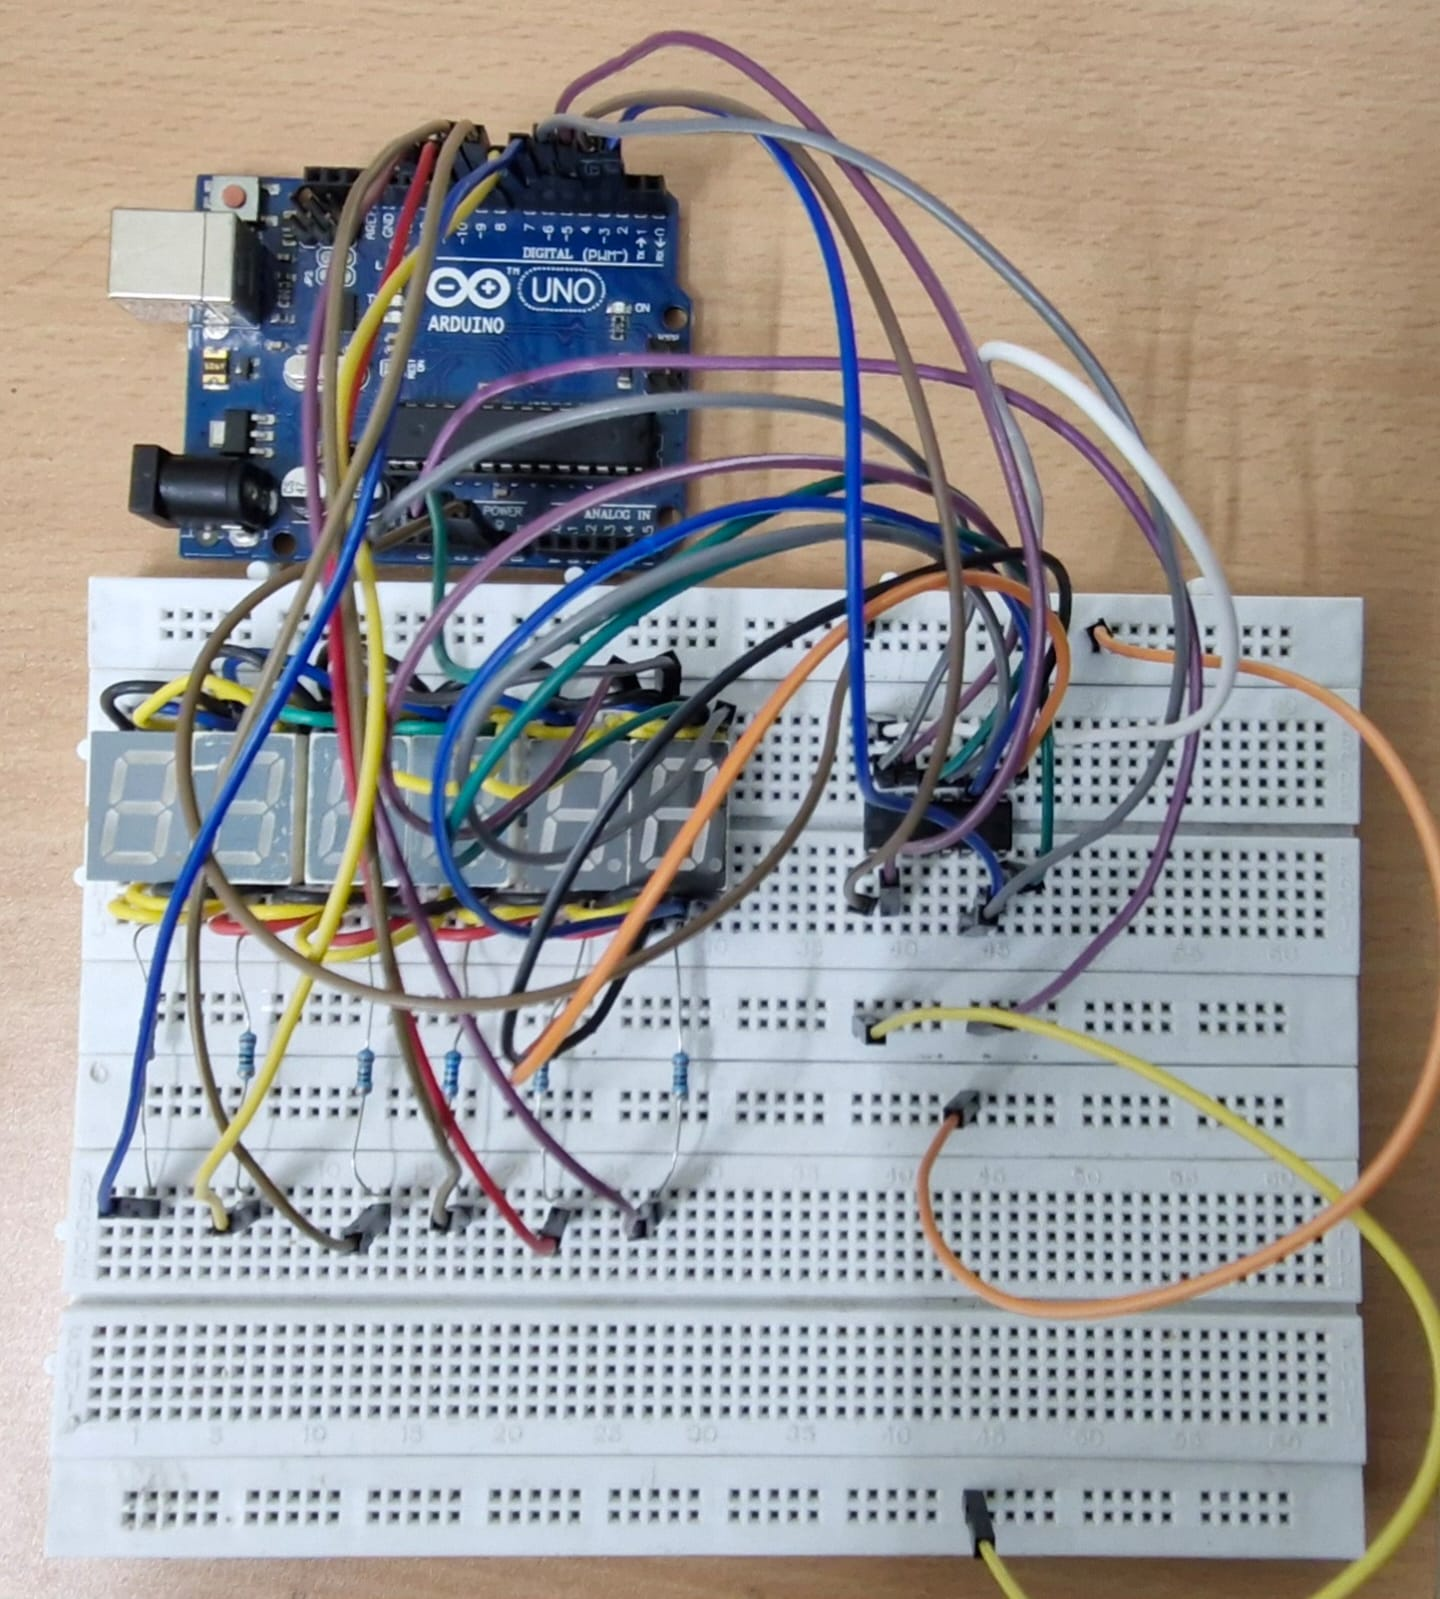
\includegraphics[width=0.5\linewidth]{figs/clockbread.jpeg}
\end{figure}

\end{document}